\break
\newpage
\section{The difference between UI \& UX. List five major current issues (within the last three years) in UX.}

\subsection{The difference between UI \& UX}
\begin{figure}[H]
    \begin{minipage}{0.3\textwidth}
        \centering
        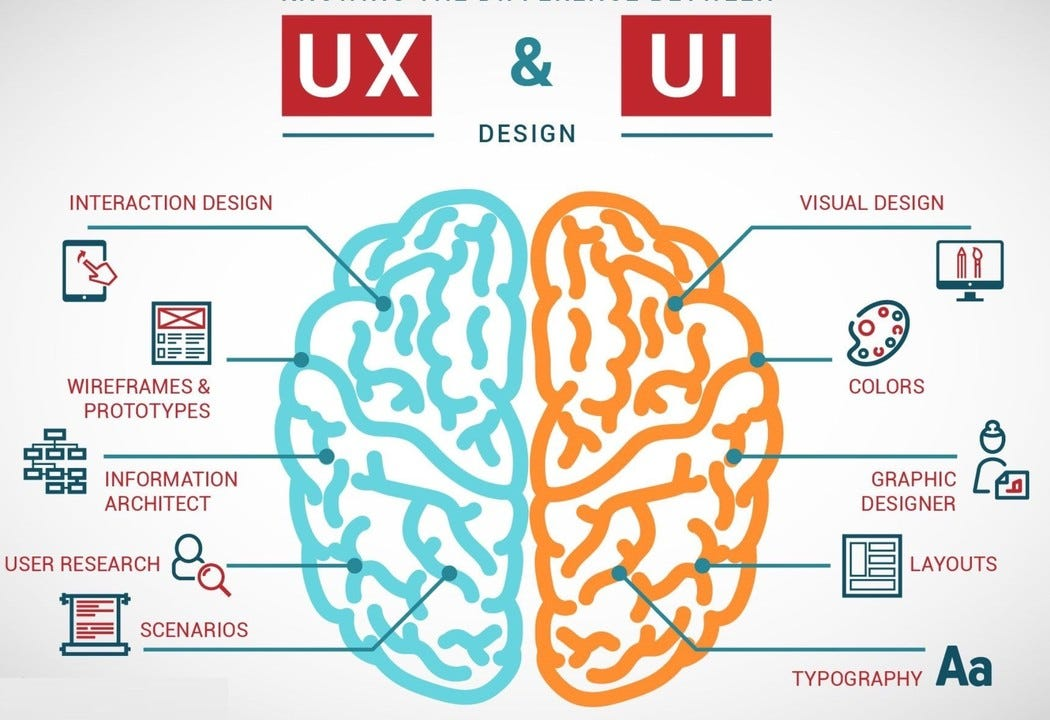
\includegraphics[width=0.8\textwidth]{img/ux-ui.jpg}
        \caption{The difference between UI \& UX}
        \label{fig:ui-ux}
    \end{minipage}
    \hfill
    \begin{minipage}{0.6\textwidth}
        \noindent
        UX defines the structural logic and experiential flow of a digital product, ensuring it addresses real user needs through research-driven design \cite{norman2013}. \\ 
        UI translates this structure into a tangible visual interface, shaping how users perceive and interact with the product through graphic and interaction design decisions \cite{garrett2011}.
    \end{minipage}
\end{figure}
\begin{table}[h]
    \centering
    \caption{The difference between UI \& UX}
    \begin{tabular}{p{4cm} p{5cm} p{5cm}}
    \hline
    \textbf{Aspect} & \textbf{UX} & \textbf{UI} \\
    \hline
    Focus & End-to-end user experience & Visual and interactive layer \\
    Key Work & Research, flows, usability & Layout, color, typography \\
    Goal & Useful and accessible products & Clear and intuitive interfaces \\
    \hline
    \end{tabular}
    \end{table}
    
    \subsection{Five major current issues in UX (2023--2025)}
    \begin{table}[H]
        \centering
        \caption{Five major current issues in UX (2023--2025)}
        \begin{tabular}{p{4cm} p{13cm}}
        \hline
        \textbf{Issue} & \textbf{Description} \\
        \hline
        \textbf{AI and Data Ethics} & Generative AI challenges privacy, authorship, and human decision-making in UX practice \cite{shneiderman2022}. \\
        \textbf{Dark Patterns} & Metric-driven design promotes manipulative interactions that erode user trust \cite{mathur2019}. \\
        \textbf{Algorithmic Personalization} & Automated personalization risks bias and loss of user agency when replacing qualitative research. \\
        \textbf{Product Quality Decline} & Rapid release cycles produce unstable experiences, undermining reliability. \\
        \textbf{Role Dilution} & UX designers face increased organizational pressure, reducing focus on evidence-based design \cite{rosenfeld2018}. \\
        \hline
        \end{tabular}
    \end{table}